\subsection{Various Payloads}
\label{sec:varioustech}
This section lists evasion techniques applicable to various payloads.

\subsubsection{Payload Size}
\label{sec:payloadsize}
Some web application firewalls are configured to skip requests sizes above a set threshold.

AWS \acrshort{waf} limits the \quotes{Maximum size of a web request body that can be inspected for CloudFront, API Gateway, Amazon Cognito, App Runner, and Verified Access protections**} to 64 KB, the \quotes{Maximum size of a web request body that can be inspected for Application Load Balancer and AWS AppSync protections} to 8 KB. \cite{aws/waflimits}

Microsoft Azure allows the configuration of limits on newer Rule Sets:
\begin{quote}
	For Application Gateway v2 Web Application Firewalls running Core Rule Set 3.2, or newer, the maximum request body size enforcement and max file upload size enforcement can be disabled and the Web Application Firewall will no longer reject a request, or file upload, for being too large. When maximum request body size enforcement and max file upload size enforcement are disabled within the Web Application Firewall, Application Gateway's limits determine the maximum size allowable. For more information, see Application Gateway limits. \cite{ms/azurewaflimits}
\end{quote}
with the \quotes{Maximum request inspection limit (\acrshort{waf} SKU)} at a default value of 2 MB with the option to disable the limit completely according to their "Application Gateway limits" document. \cite{ms/appgatewaylimits}

Akamai answers the question \quotes{Can [a] \acrshort{waf} inspect all arguments and values in [the] request body? Is there any limitation on the size of the request?} on their \acrshort{faq} page with \quotes{By default, the \acrshort{waf} inspects only the first 8KB of a request. It can increase the limit up to 128KB by adding Advanced Metadata.} \cite{akamai/waflimits}

Cloudflare lists a limit of 128 KB in the Cloudflare Rules language definition, with truncation upon reaching it:
\begin{quote}
	All http.request.body.* fields (except http.request.body.size) handle a maximum body size of 128 KB, which means that you cannot define expressions that rely on request body data beyond the first 128 KB. If the request body is larger, the body fields will contain a truncated value and the http.request.body.truncated field will be set to true. The http.request.body.size field will contain the full size of the request without any truncation.

	The maximum body size of 128 KB applies only to the values of \acrshort{http} body fields — the origin server will still receive the complete request body. \cite{cloudflare/limits}
\end{quote}

The ModSecurity recommended configuration sets the following limits for requests:
\begin{quote}
	SecRequestBodyLimit 13107200 \\
	SecRequestBodyNoFilesLimit 131072
\end{quote}
with requests exceeding the limits being rejected by default. \cite{modsec/recconf}

Depending on the specific rule configuration by each service, filling up requests with filler data to exceed the inspection limit might make the malicious payload evade detection. Some web applications might accept request bodies filled with unused data, as long as there is a valid key: value pair inside. If this key: value pair is positioned past the 8 KB limit of the Akamai \acrshort{waf} for instance, the malicious value might go unnoticed. Results of using this technique during the evaluation are stated under Section~\ref{sec:paylensingleiter}.


\subsubsection{Unicode Escaping in JSON}
\label{sec:unicodeinjson}
RFC 4627 \quotes{The application/json Media Type for JavaScript Object Notation} states under section 2.5 \quotes{Strings}:
\begin{quote}
	The representation of strings is similar to conventions used in the C
	family of programming languages.  A string begins and ends with
	quotation marks.  All Unicode characters may be placed within the
	quotation marks except for the characters that must be escaped:
	quotation mark, reverse solidus, and the control characters (U+0000
	through U+001F).

	Any character may be escaped.  If the character is in the Basic
	Multilingual Plane (U+0000 through U+FFFF), then it may be
	represented as a six-character sequence: a reverse solidus, followed
	by the lowercase letter u, followed by four hexadecimal digits that
	encode the character's code point.  The hexadecimal letters A though
	F can be upper or lowercase.  So, for example, a string containing
	only a single reverse solidus character may be represented as
	"\verb|\u005C|". \cite{rfc4627}
\end{quote}
As escaping any character should be possible in a JSON payload, firewall filters that look for a certain sequence of characters might be evaded by escaping one or more characters from that sequence. Messages exchanged between web clients and web servers are often in JSON format. As such, sometimes the JSON format is used when crafting messages containing malicious payloads. In this case, any character inside the JSON formatted message can be escaped using this technique. For example, a payload inside the JSON formatted body of a \acrshort{http} message:

\begin{lstlisting}[style=basicStyle, language=Python]
{
	"message": "alert(\"JSON\")"
}
\end{lstlisting}

To evade a filter looking for the character sequence \verb|alert(|, the payload inside the message may be modified to:

\begin{lstlisting}[style=basicStyle, language=Python]
{
	"message": "alert\u0028\"JSON\")"
}
\end{lstlisting}

The JSON parser does not differentiate between both payloads. As such, the following statements running inside a web browser are semantically equal:

\begin{lstlisting}[style=basicStyle, language=Python]
eval(JSON.parse('{"message":"alert(\\"JSON\\")"}').message)

eval(JSON.parse('{"message":"alert\\u0028\\"JSON\\")"}').message)
\end{lstlisting}

Results of using this technique during the evaluation are stated under Section~\ref{sec:unicodeinjsontest} and Section~\ref{sec:forcedunicodenorm}.


\subsubsection{Unicode Normalization}
\label{sec:unicodenormalization}
The unicode standard defines two types of equivalence between characters: canonical equivalence and compatibility equivalence. The report "Unicode Normalization Forms" by Ken Whistler for Unicode Version 15.1.0 states the following regarding the two types of equivalence:

\begin{quote}
	Canonical equivalence is a fundamental equivalency between characters or sequences of characters which represent the same abstract character, and which when correctly displayed should always have the same visual appearance and behavior. Figure 1 shows this type of equivalence with examples of several subtypes.
	\\
	\begin{figure}[h]
		\centering
		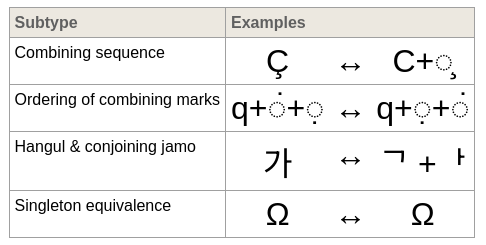
\includegraphics[width=0.5\textwidth]{caneq.png}
		\label{fig:caneq}
		\caption{ Examples of Canonical Equivalence \cite{unicode/normalization}}
	\end{figure}
	\\
	Compatibility equivalence is a weaker type of equivalence between characters or sequences of characters which represent the same abstract character (or sequence of abstract characters), but which may have distinct visual appearances or behaviors. The visual appearances of the compatibility equivalent forms typically constitute a subset of the expected range of visual appearances of the character (or sequence of characters) they are equivalent to. However, these variant forms may represent a visual distinction that is significant in some textual contexts, but not in others. As a result, greater care is required to determine when use of a compatibility equivalent is appropriate. [...] Figure 2 provides examples of compatibility equivalence. \cite{unicode/normalization}
	\begin{figure}[!h]
		\centering
		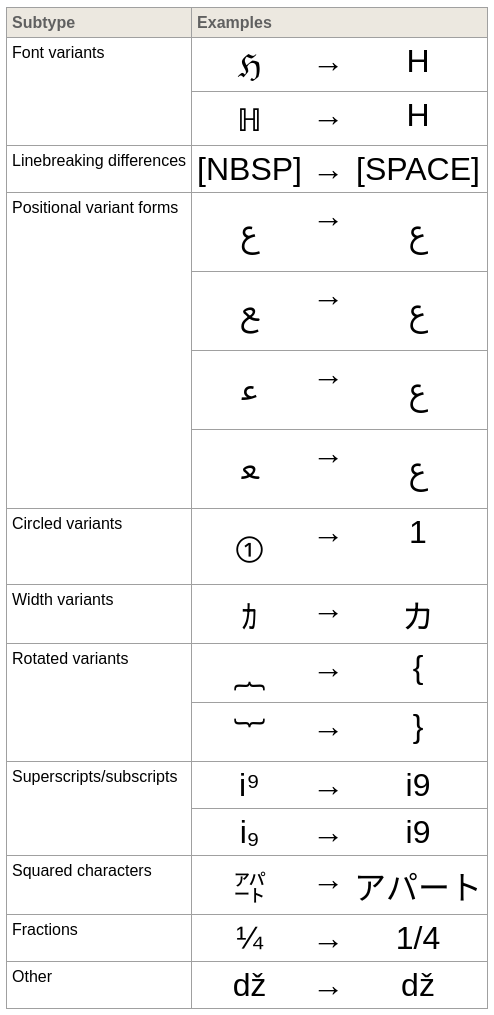
\includegraphics[width=0.5\textwidth]{compeq.png}
		\label{fig:compeq}
		\caption{ Examples of Compatibility Equivalence \cite{unicode/normalization}}
	\end{figure}
\end{quote}

Regarding Normalization Forms, the report states in further proceedings:
\begin{quote}
	Unicode Normalization Forms are formally defined normalizations of Unicode strings which make it possible to determine whether any two Unicode strings are equivalent to each other. Depending on the particular Unicode Normalization Form, that equivalence can either be a canonical equivalence or a compatibility equivalence.

	Essentially, the Unicode Normalization Algorithm puts all combining marks in a specified order, and uses rules for decomposition and composition to transform each string into one of the Unicode Normalization Forms. A binary comparison of the transformed strings will then determine equivalence.

	The four Unicode Normalization Forms are summarized in Table 1. \cite{unicode/normalization}
\end{quote}
\begin{table}
	\centering
	\label{tab:normform}
	\caption{ Normalization Forms }
	\begin{tabular}{ |c|c| }
		\hline
		Form                         & Description                       \\
		\hline
		\hline
		Normalization Form D (NFD)   & Canonical Decomposition           \\
		\hline
		Normalization Form C (NFC)   & Canonical Decomposition,          \\
		                             & followed by Canonical Composition \\
		\hline
		Normalization Form KD (NFKD) & Compatibility Decomposition       \\
		Normalization Form KC (NFKC) & Compatibility Decomposition,      \\
		                             & followed by Canonical Composition \\
		\hline
	\end{tabular}
\end{table}
In the context of Firewall Evasion, if inputs on the web server are normalized using one of the afromentioned Normalization Forms during processing, an attacker could try to substitute certain characters inside a malicious payload with equivalent unicode characters. \cite{medium/allypetitt}
Such a payload might be able to avoid the filter of the web Application Firewall that is looking for patterns including only the normalized form of the unicode character. As an example, the payload:

\begin{lstlisting}[style=basicStyle, language=Python]
"prompt`${secret}`"
\end{lstlisting}

could be substituted with the payload:

\begin{lstlisting}[style=basicStyle, language=Python]
"prompt`\uFE69{secret}`"
\end{lstlisting}

The unicode character U+FE69 is named "Small Dollar Sign" and its decomposition form is U+0024, which is the regular Dollar Sign. \cite{comp/uni}

Using the JavaScript function \verb|normalize()|, the string containing the Small Dollar Sign: \verb|"\uFE69"| can be decomposed using Compatibility Decomposition (NFKD) into a string containing the normal Dollar Sign: \verb|"\u0024"| respectively \verb|"$"|.
By calling \verb|.normalize("NFKD")| on the afromentioned example payload:

\begin{lstlisting}[style=basicStyle, language=Python]
"prompt`\uFE69{secret}`".normalize("NFKD")
\end{lstlisting}

the payload will be normalized to the initial payload:

\begin{lstlisting}[style=basicStyle, language=Python]
"prompt`${secret}`"
\end{lstlisting}

If the web application evaluates the payload post normalization, the target effect has been achieved by the antagonist actor. An example of a vulnerable function inside a web application is given in the following code sample. Consider the variable \verb|incomingPayload| to be holding the incoming payload:

\begin{lstlisting}[style=basicStyle, language=Python, caption=vulnerable through Unicode Normalization code sample]
const secret = "very secret string"
const incomingPayload = "a\");prompt`\uFE69{secret}`;(\""
const message = "Hello " + incomingPayload.normalize('NFKD')
const evaluateMe = "console.log(\"" + message + "\")"
eval(evaluateMe)
\end{lstlisting}

Unicode Normalization is also supported in programming languages different to JavaScript, such as Python. \cite{python/normalization}

Results of evaluated payloads obscured using this technique are stated under Section~\ref{sec:uninormsingleiter} and Section~\ref{sec:forcedunicodenorm}.


\subsubsection{Case Alternation}
\label{sec:casealt}
In order to evade regex filerting by the web application firewall, the case of a payload can be alternated. \cite{medium/allypetitt}

Modern regex flavors allow the application of modifiers to parts of the regular expression.
One such modifier is \verb|(?i)|. It makes the regex case insensitive. \cite{regex/jan} Only when this modifier is not used, can a payload evade regex filtering using case alternation.
Taking the Cross-site scripting payload:

\begin{lstlisting}[style=basicStyle, language=Python]
<script>alert('XSS')</script>
\end{lstlisting}

as an example. After applying case alternation, it might result in a payload in the form of:

\begin{lstlisting}[style=basicStyle, language=Python]
<sCrIpT>alert('XSS')</sCriPt>
\end{lstlisting}

Another example is file access on a wrongfully public file.
The Windows file system treats file and directory names as case-insensitive by default. \cite{windows/casesensitive} On a web server hosted on Windows that exposes a .env file with stored secrets, the url:

\begin{lstlisting}[style=basicStyle, language=Python]
http://127.0.0.1:8000/.env
\end{lstlisting}

is treated equally to the url:

\begin{lstlisting}[style=basicStyle, language=Python]
http://127.0.0.1:8000/.enV
\end{lstlisting}

Results of conducting the evaluation using this technique are stated under Section~\ref{sec:casealternationevaluation}.



% \subsubsection{Comment interference}
% \label{sec:commint}
% {\color{red} TODO: rework this to javascript comment interference}

% In some context, comments can be used to break up statements. Regarding SQL, the Oracle Database SQL Reference states:
% \begin{quote}
% 	A comment can appear between any keywords, parameters, or punctuation marks in a statement. You can include a comment in a statement in two ways:
% 	\begin{itemize}
% 		\item Begin the comment with a slash and an asterisk (/*). Proceed with the text of the comment. This text can span multiple lines. End the comment with an asterisk and a slash (*/). The opening and terminating characters need not be separated from the text by a space or a line break.
% 		\item Begin the comment with -- (two hyphens). Proceed with the text of the comment. This text cannot extend to a new line. End the comment with a line break.
% 	\end{itemize}
% 	\cite{oracle/sqlcomments}
% \end{quote}
% Ally Petitt suggests using comments inside SQL statements to break up SQL keywords: \verb|?id=1+un/**/ion+sel/**/ect+1,2,3--| \cite{medium/allypetitt}


\subsubsection{Percent Encoding}
\label{sec:percenc}
RFC 3986 states under section 2.1 "Percent-Encoding":
\begin{quote}
	A percent-encoding mechanism is used to represent a data octet in a
	component when that octet's corresponding character is outside the
	allowed set or is being used as a delimiter of, or within, the
	component.  A percent-encoded octet is encoded as a character
	triplet, consisting of the percent character "\%" followed by the two
	hexadecimal digits representing that octet's numeric value.  For
	example, "\%20" is the percent-encoding for the binary octet
	"00100000" (ABNF: \%x20), which in US-ASCII corresponds to the space
	character (SP). \cite{rfc3986}
\end{quote}
If a web application firewall does not perform percent-decoding on filtered requests but the request is being decoded by the web server, such as is the case when data is being sent as part of an \acrshort{uri} (\cite{rfc3986/sec2.4}), a malicious payload could be percent-encoded to avoid detection by the firewall.

The payload:

\begin{lstlisting}[style=basicStyle, language=Python]
<script>alert('XSS')</script>
\end{lstlisting}

becomes

\begin{lstlisting}[style=basicStyle, language=Python]
%3Cscript%3Ealert%28%27XSS%27%29%3C%2Fscript%3E
\end{lstlisting}

after percent encoding it with the Python function \verb|urllib.parse.quote_plus|. Evaluation results using this technique are stated under Section~\ref{sec:percencsingleiter}, Section~\ref{sec:doublepercenc}, Section~\ref{sec:jsencpercenc} and Section~\ref{sec:forcedunicodenorm}.


\subsubsection{Charset Alternation}
\label{sec:charsetalt}
To indicate the original media type prior to any applied content encoding, the \acrshort{http} \verb|Content-Type| representation header is used.
It can be used in requests by the client to tell the server what type of data is actually sent.
\verb|charset| is a possible directive, that can be supplied with the \verb|Content-Type| header.
It specifies the character encoding standard. \cite{http/contenttype}
If a web server is supporting requests in different encoding standards, but the web application firewall is not configured to parse certain encoding standards, the web application firewall may not recognize such encoded request as malicious.

If the payload:

\begin{lstlisting}[style=basicStyle, language=Python]
<script>alert("xss")</script>
\end{lstlisting}

is encoded to the charset \verb|UTF-16|, as stated in the Python 3 code sample:

\begin{lstlisting}[style=basicStyle, language=Python]
pl = "<script>alert('xss')</script>"
ex_encoding = 'UTF-16'
pl_encoded = pl.encode(ex_encoding)
\end{lstlisting}

it becomes:

\begin{lstlisting}[style=basicStyle]
\xff\xfe<\x00s\x00c\x00r\x00i\x00p\x00t\x00>\x00a\x00l\x00e\x00r\x00t\x00(\x00'\x00x\x00s\x00s\x00'\x00)\x00<\x00/\x00s\x00c\x00r\x00i\x00p\x00t\x00>\x00
\end{lstlisting}

This payload differs from the original payload in \verb|UTF-8|. \verb|UTF-8| encoding is the standard for \acrshort{uri}s according to RFC-3986. \cite{rfc3986}

If a web server accepts \acrshort{http} requests in \verb|UTF-16| encoding and the web application firewall does not recognize payloads encoded in \verb|UTF-16|, any payload can be sent towards the web application without being detected by the web application firewall. Results of testing this technique during the evaluation are stated under Section~\ref{sec:charaltsingleiter}.

This technique is proposed by Ally Petitt. \cite{medium/allypetitt}
